\documentclass{subfiles}

\begin{document}
    \marginnote{\textbf{\textit{VL 10}}\\16.05.2023, 11:45}[-0.5cm]

    Für die Ebene Welle $C_0\cdot\text{exp}(\cmath \cdot\scpr{k}{x})$ folgt analog $j(t,x) = \abs{C_0}^2\cdot \hbar\cdot k / m$. 
    \begin{Aufgabe}
        \nr{} Verifiziere $\abs{\rho}_\C^2 + \abs{\tau}_\C^2 = 1$. Was ist die physikalisch anschauliche Begründung?
    \end{Aufgabe}
    In der Fourierform haben wir den Identitätszusammenhang
    \[\psi(t,x) = (\mcF^{-1}\circ\mcF)\psi(t,x).\]
    \begin{Aufgabe}
        \nr{} Berechne für die obige eindimensionale zeitunabhängige Lösung $\psi(t,x)$ die Fouriertransformierte $\mcF\psi(t,x)=:\hat\psi(p)$. 
    \end{Aufgabe}
    Mit der obigen Aufgabe folgt dann, daß der Impuls $p$ über die Zeit nicht erhalten ist; also $\overline p\neq p$ und in der Sprache des Kommutators $[p,H]\neq 0$. Optisch erhalten wir für die Wahrscheinlichkeitsverteilung eine \emph{Aufspaltung} in zwei Peaks; Das Teilchen selbst ist allerdings nicht aufgespalten - die Implikation an dieser Stelle gilt also nicht. 
    \begin{figure}[H]
        \centering
        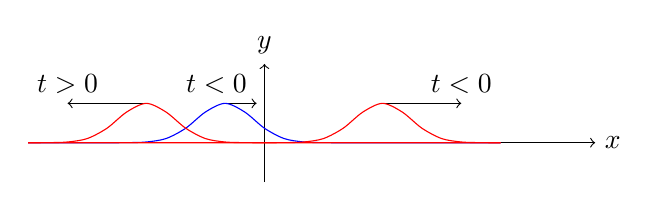
\begin{tikzpicture}
            \draw[->] (-3, 0) -- (4.2, 0) node[right] {$x$};
            \draw[->] (0, -0.5) -- (0, 1) node[above] {$y$};

            \draw[->] (-1.5, 0.5) -- (-2.5, 0.5) node[above] {$t>0$};
            \draw[->] (1.5, 0.5) -- (2.5, 0.5) node[above] {$t<0$};
            \draw[->] (-0.5,0.5) -- (-0.1,0.5) node[above left] {$t<0$};

            \draw[scale=0.5, domain=-6:6, smooth, variable=\x, blue] plot ({\x}, {exp(-(\x + 1)^2)});
            \draw[scale=0.5, domain=-6:6, smooth, variable=\x, red]  plot ({\x}, {exp(-(\x - 3)^2)});
            \draw[scale=0.5, domain=-6:6, smooth, variable=\x, red]  plot ({\x}, {exp(-(\x + 3)^2)});
        \end{tikzpicture}
        \caption{Wahrscheinlichkeitsverteilung zu $t<0$ (blau) und $t>0$ (rot).}
    \end{figure}
    Wir führen nun eine Abkürzung für die allgemeine Lösung des zeitunabhängigen eindimensionalen Problems ein:
    \[u_{f,x_0}(t,x):=\begin{cases}
        f_+(t,x) + \rho\cdot f_-(t,x) & x\leq x_0 \\
        \tau\cdot f_\kappa(t,x) & x>x_0
    \end{cases},\]
    wobei der Buchstabe $f$ eine Erinnerung an entsprechende Funktionen $f_-,f_+,f_\kappa$ ist. 
    \begin{Aufgabe}
        \nr{} Überlege dir die Übersetzungsfunktionen $f_+,f_-,f_\kappa$ für die oben erhaltene explizite Lösung. 
    \end{Aufgabe}
    Beachtlich ist nun, daß das quantenmechanische Teilchen mit einer Wahrscheinlichkeit $>0$ auf der rechten Seite der Potentialbarriere vorfindbar ist; dies ist Resultat der Heisenbergschen Unschärferelation:
    \[(\Delta x)_{u_{\exp,0}}\circ(\Delta H)_{u_{\exp,0}}\geq \frac{1}{2}\abs{\langle[H,x]\rangle_{u_{\exp,0}}} = \frac{\hbar\cdot\langle p\rangle_{u_{\exp,0}}}{2\cdot m}\neq 0.\]
    Daraus folgt für eine Unschärfe $(\Delta x)_{u_{\exp,0}}>0$ eine Unschärfe $(\Delta H)_{u_{\exp,0}} \approx p^2/(2m)$, sodaß $\hbar/\overline p = 1/\kappa$. 
    

\end{document}